%%%%%%%%%%%%%%%%%%%%%%%%%%%%%%%%%%%%%%%%%%%%%%%%%%%%%%%%%%%%%%%%%%%%%%
%%%%%%%%%%%%%%%%%%%%%%%%%%%%%%%%%%%%%%%%%%%%%%%%%%%%%%%%%%%%%%%%%%%%%%
\documentclass[dvips,portrait]{seminar}             %%%%%%%%%%%%%%%%%%
                                                    %%%%%%%%%%%%%%%%%%
%%%%%%%%%%%%%%%%%%%%%%%%%%%%%%%%%%%%%%%%%%%%%%%%%%%%
% gmake afb-sig-ps
%======================
\input Energy.tex
%\def\Energy{MZ-1.8GeV (had.)}
\def\Angle{$\theta^{\bullet}$}

%%%%%%%%%%%%%%%%%%%%%%%%%%%%%%%%%%%%%%%%%%%%%%%%%%%%%%%
%%%%%%%%%%%%%%%%%%%%%%%%%%%%%%%%%%%%%%%%%%%%%%%%%%%%%%%
\begin{document}                     %%%%%%%%%%%%%%%%%%


%//////////////////////////////////////////////////////////////////////////////////
%//////////////////////////////////////////////////////////////////////////////////
%//////////////////////////////////////////////////////////////////////////////////
\begin{slide}
\titbox{{\bf\Color{Red} CEEX $\sigma$ and $A_{\rm FB}$, energy cut-off study }}

\setlength{\unitlength}{1mm}
{\small\Color{PineGreen}
  Process: $e^-e^+ \to f\bar{f}$, $f=\mu^-$, at \Energy.
  Energy cut: $v<v_{\max}$, where $v=1-M^2_{f\bar{f}}/s$.
  Scattering angle for $A_{\rm FB}$ is $\theta=$\Angle.
  No cut in \Angle. 
  E-W corr. in \KK\  according to DIZET 6.x.
  \OrderLL{\alpha^3} EEX3 matrix element in \KK\ (without ISR*FSR interf.)
  \KK{}sem is semianalytical part of \KK.
  {\tiny (Angle $\theta^{\bullet}$ is from Phys. Rev. {\bf D41}, 1425 (1990).)}
}
\begin{picture}(105,54)
\put(-2, 00){\makebox(0,0)[lb]{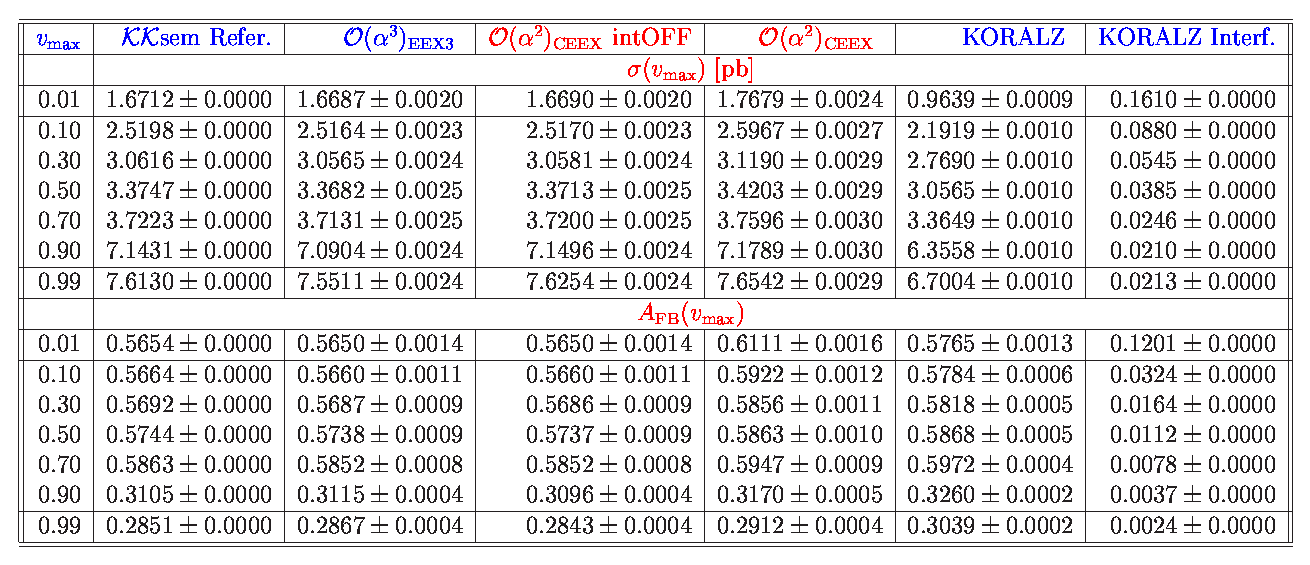
\epsfig{file=afb-int-tab1.eps,width=105mm,height=54mm}}}
\end{picture}
%-----------------------------------------------------------
\vfill
\end{slide}   %%%
%%%%%%%%%%%%%%%%%%



%//////////////////////////////////////////////////////////////////////////////////
%//////////////////////////////////////////////////////////////////////////////////
%//////////////////////////////////////////////////////////////////////////////////
\begin{slide*}
\titbox{{\large\bf\Color{Magenta} Total cross section $\sigma$, energy cut-off stydy}}

{\small\Color{Blue}
  The same as in the table.
  The {\Color{Red} ISR$\otimes$FSR  interf.} switched on/off wherever possible.
  No cut in \Angle.
  Reference $\sigma_{\rm ref}$ = semianalytical of \KK{}sem,
  (no ISR$\otimes$FSR,  up to \OrderLL{\alpha^3}, JSW exponentiation).
  EEX2 data points from KORALZ/YFS3 version 4.03 
  (QED up to \OrderLL{\alpha^2}, ISR$\otimes$FSR off).
}
\begin{center}
\setlength{\unitlength}{1mm}
\begin{picture}(70,60)
%#####\put(0,0){\framebox( 70,60){ }}
\put(-2, 00){\makebox(0,0)[lb]{
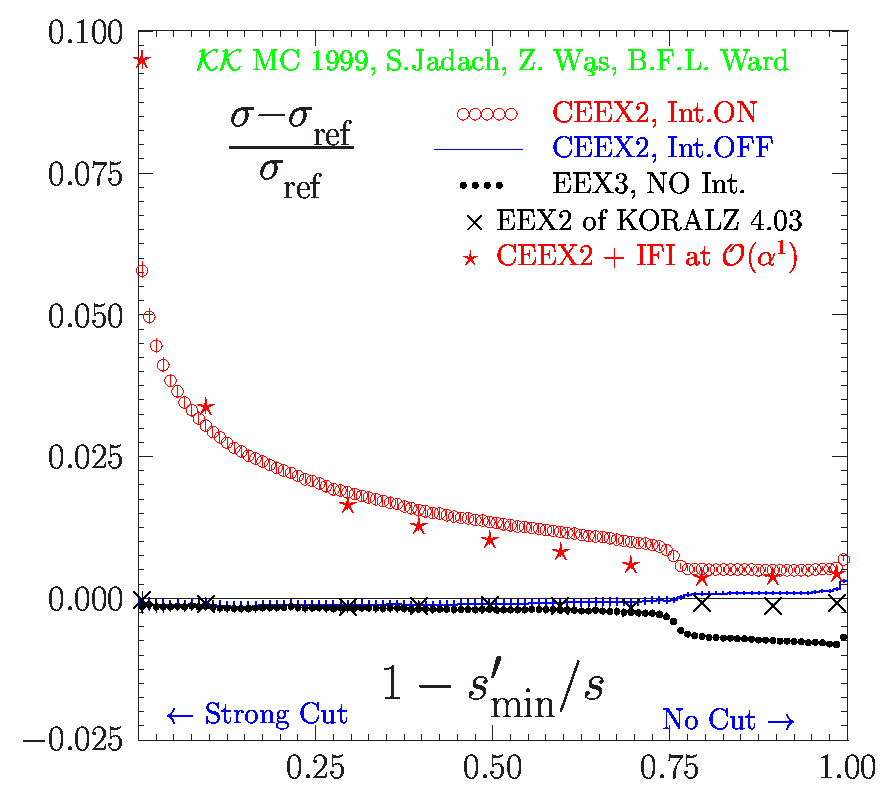
\epsfig{file=afb-int-Gsig.eps,width=70mm,height=60mm}
}}
\end{picture}
\end{center}
%-----------------------------------------------------------
\vfill
\end{slide*}   %%%
%%%%%%%%%%%%%%%%%%



%//////////////////////////////////////////////////////////////////////////////////
%//////////////////////////////////////////////////////////////////////////////////
%//////////////////////////////////////////////////////////////////////////////////
\begin{slide*}
\titbox{{\large\bf\Color{Magenta} Charge asymmetry $A_{\rm FB}$, energy cut-off study}}

{\small\Color{Blue}
  The same as in the table.
  The {\Color{Red} ISR$\otimes$FSR  interf.} switched on/off wherever possible.
  No cut in \Angle.
  Reference $A_{\rm FB}^{\rm ref}$ =  semianalytical \KK{}sem,
  (no ISR$\otimes$FSR,  up to \OrderLL{\alpha^3}, JSW exponentiation).
  EEX2 data points are from KORALZ/YFS3 version 4.03 
  (QED up to \OrderLL{\alpha^2}, ISR$\otimes$FSR off.).
}

\begin{center}
\setlength{\unitlength}{1mm}
\begin{picture}(75,60)
%#####\put(0,0){\framebox( 75,60){ }}
\put(-2, 00){\makebox(0,0)[lb]{
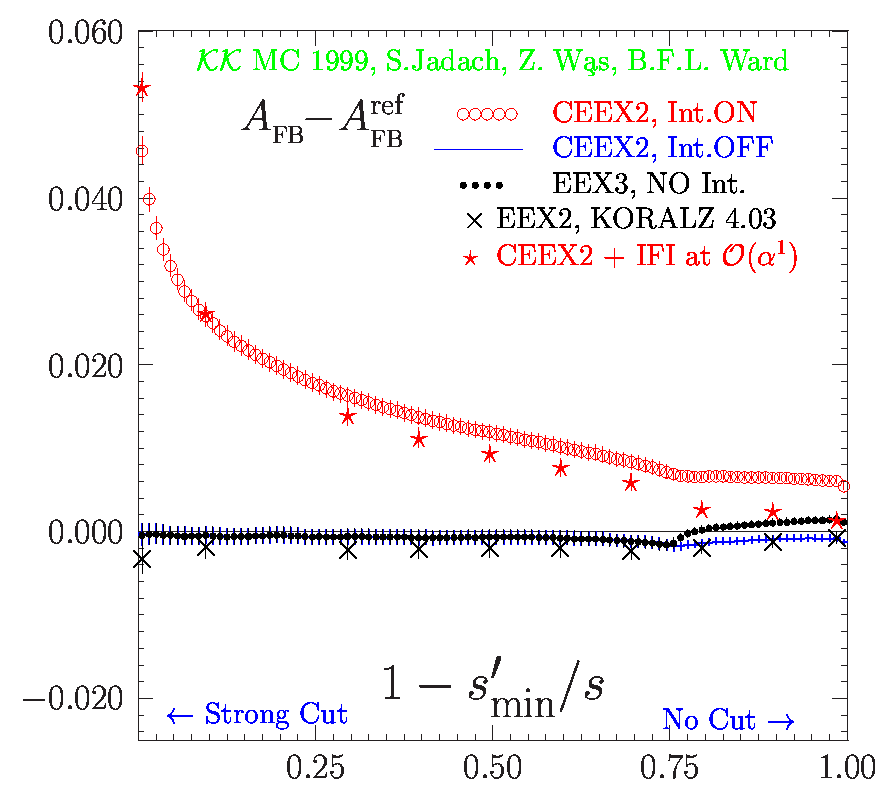
\epsfig{file=afb-int-Gafb.eps,width=75mm,height=60mm}
}}
\end{picture}
\end{center}
%-----------------------------------------------------------
\vfill
\end{slide*}   %%%
%%%%%%%%%%%%%%%%%%



%//////////////////////////////////////////////////////////////////////////////////
%//////////////////////////////////////////////////////////////////////////////////
%//////////////////////////////////////////////////////////////////////////////////
\begin{slide*}
\titbox{{\large\bf\Color{Magenta} Total x-section $\sigma$, comparison with Zfitter}}

{\Color{Blue}
  Comparison with Zfitter 6.xx.
  The {\Color{Red} ISR$\otimes$FSR  interf.} switched on/off.
  No cut in $\theta_1$.
  Reference $\sigma_{\rm ref}$ = semianalytical of \KK{}sem,
  (no ISR$\otimes$FSR,  up to \OrderLL{\alpha^3}, JSW exponentiation).
}
\begin{center}
\setlength{\unitlength}{1mm}
\begin{picture}(70,60)
%#####\put(0,0){\framebox( 70,60){ }}
\put(-2, 00){\makebox(0,0)[lb]{
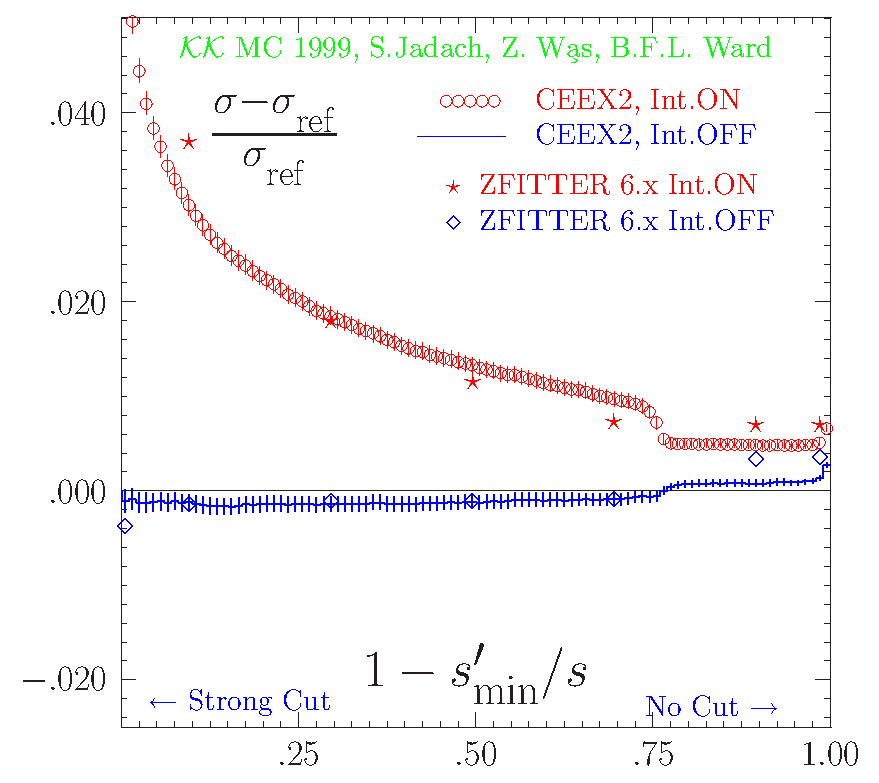
\epsfig{file=afb-int-GsigZFtheta1.eps,width=70mm,height=60mm}
}}
\end{picture}
\end{center}
%-----------------------------------------------------------
\vfill
\end{slide*}   %%%
%%%%%%%%%%%%%%%%%%



%//////////////////////////////////////////////////////////////////////////////////
%//////////////////////////////////////////////////////////////////////////////////
%//////////////////////////////////////////////////////////////////////////////////
\begin{slide*}
\titbox{{\large\bf\Color{Magenta} Charge asymmetry $A_{\rm FB}$, comparison with Zfitter}}

{\Color{Blue}
  Comparison with Zfitter 6.xx.
  The {\Color{Red} ISR$\otimes$FSR  interf.} switched on/off.
  No cut in $\theta_1$.
  Reference $A_{\rm FB}^{\rm ref}$ =  semianalytical \KK{}sem,
  (no ISR$\otimes$FSR,  up to \OrderLL{\alpha^3}, JSW exponentiation).
}

\begin{center}
\setlength{\unitlength}{1mm}
\begin{picture}(75,60)
%#####\put(0,0){\framebox( 75,60){ }}
\put(-2, 00){\makebox(0,0)[lb]{
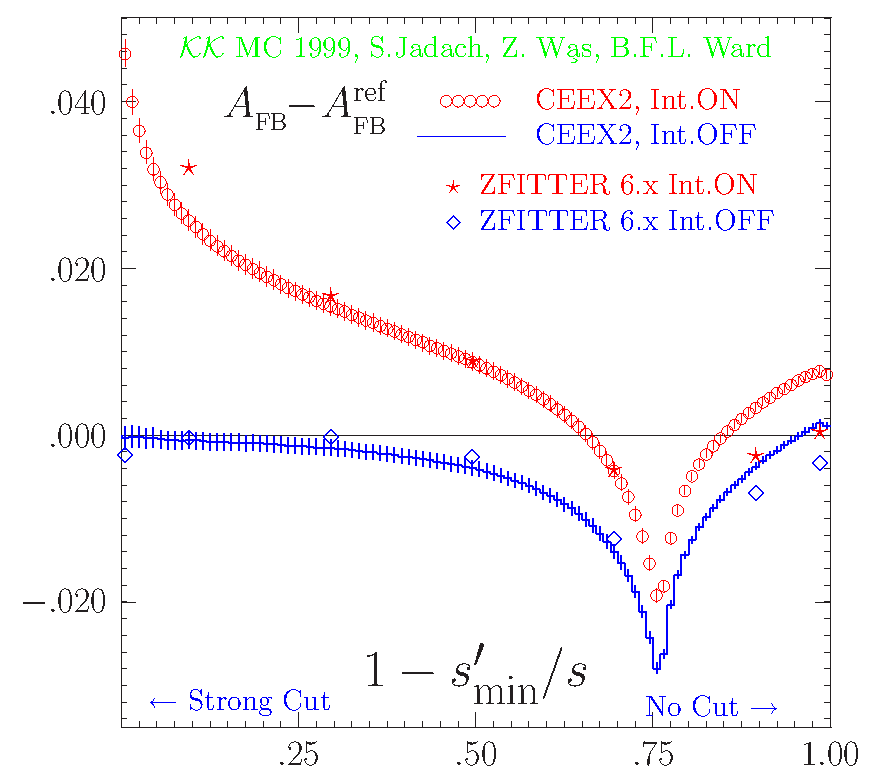
\epsfig{file=afb-int-GafbZFtheta1.eps,width=75mm,height=60mm}
}}
\end{picture}
\end{center}
%-----------------------------------------------------------
\vfill
\end{slide*}   %%%
%%%%%%%%%%%%%%%%%%


%//////////////////////////////////////////////////////////////////////////////////
%//////////////////////////////////////////////////////////////////////////////////
%//////////////////////////////////////////////////////////////////////////////////
\begin{slide*}
\titbox{{\large\bf\Color{Magenta} 
                      Physical Precision of CEEX, NEW!!! }}

{\small\Color{Blue}
  The difference between second and first order CEEX results for at \Energy.\\
  The energy cut is on $s'/s$, where $s'=m^2_{f\bar{f}}$.}\\
{\small\Color{Blue} Scattering angle is $\theta=$\Angle. }\\
{\tiny\Color{Blue}  [Angle $\theta^{\bullet}$ is defined in Phys. Rev. {\bf D41}, 1425 (1990)]}

%-----------------------------------------------------------
\begin{center}
\setlength{\unitlength}{1mm}
%
\begin{picture}(35,35)
\put(-1, 0){\makebox(0,0)[lb]{
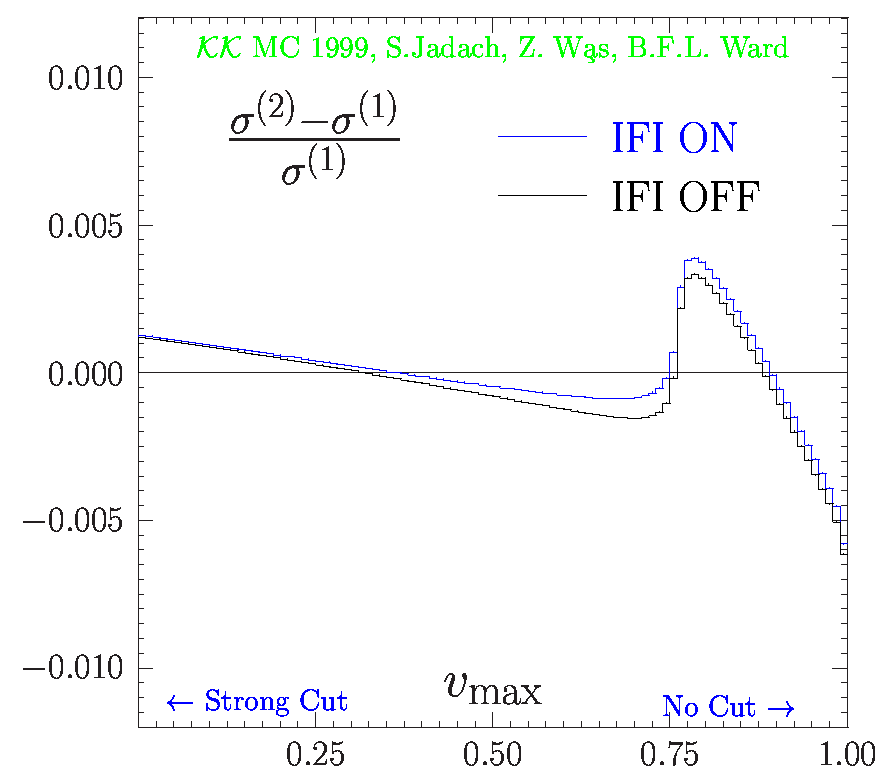
\epsfig{file=afb-int-sigHO.eps,width=35mm,height=34mm}
}}\end{picture}
%
\begin{picture}(35,35)
\put(-1, 0){\makebox(0,0)[lb]{
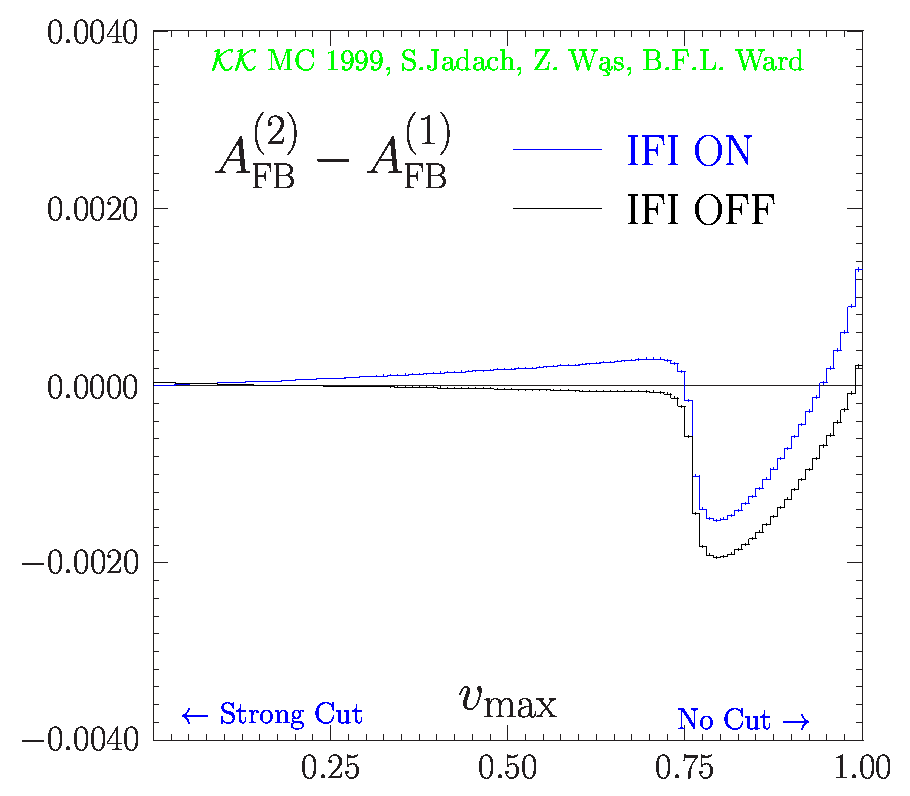
\epsfig{file=afb-int-afbHO.eps,width=35mm,height=34mm}
}}\end{picture}
\vfill
\end{center}
%-----------------------------------------------------------
\vfill
\end{slide*}   %%%
%%%%%%%%%%%%%%%%%%





\end{document}

